%
% A header that lets you compile a chapter by itself, or inside a larger document.
% Adapted from http://stackoverflow.com/questions/3655454/conditional-import-in-latex
%
%
%Use \inbpdocument and \outbpdocument in your individual files, in place of \begin{document} and \end{document}. In your main file, put in a \def \ismaindoc {} before including or importing anything.
%
% David Duvenaud
% June 2011
% 
% ======================================
%
%


\ifx\ismaindoc\undefined
	\newcommand{\inbpdocument}{
		\def \ismaindoc {}
		% Use this header if we are compiling by ourselves.
		\documentclass[a4paper,11pt,authoryear,index]{common/PhDThesisPSnPDF}
		
%\usepackage{draftwatermark}
%\SetWatermarkLightness{0.95}

% ******************************************************************************
% ****************************** Custom Margin *********************************

% Add `custommargin' in the document class options to use this section
% Set {innerside margin / outerside margin / topmargin / bottom margin}  and
% other page dimensions

\ifsetMargin
\else
    \RequirePackage[left=37mm,right=30mm,top=35mm,bottom=30mm]{geometry}
    \setFancyHdr % To apply fancy header after geometry package is loaded
\fi


%\chead{Unfinished draft}
%\cfoot{\texttt{Unfinished draft - compiled on \today{} at \currenttime}}

% *****************************************************************************
% ******************* Fonts (like different typewriter fonts etc.)*************

% Add `customfont' in the document class option to use this section

\ifsetFont
\else
    % Set your custom font here and use `customfont' in options. Leave empty to
    % load computer modern font (default LaTeX font).  

    \RequirePackage{libertine} 
\fi

% *****************************************************************************
% *************************** Bibliography  and References ********************

%\usepackage{cleveref} %Referencing without need to explicitly state fig /table

% Add `custombib' in the document class option to use this section
\ifsetBib % True, Bibliography option is chosen in class options
\else % If custom bibliography style chosen then load bibstyle here

   \RequirePackage[square, sort, numbers, authoryear]{natbib} % CustomBib

% If you would like to use biblatex for your reference management, as opposed to the default `natbibpackage` pass the option `custombib` in the document class. Comment out the previous line to make sure you don't load the natbib package. Uncomment the following lines and specify the location of references.bib file

% \RequirePackage[backend=biber, style=numeric-comp, citestyle=numeric, sorting=nty, natbib=true]{biblatex}
% \bibliography{References/references} %Location of references.bib only for biblatex

\fi


% changes the default name `Bibliography` -> `References'
\renewcommand{\bibname}{References}


% *****************************************************************************
% *************** Changing the Visual Style of Chapter Headings ***************
% Uncomment the section below. Requires titlesec package.

%\RequirePackage{titlesec}
%\newcommand{\PreContentTitleFormat}{\titleformat{\chapter}[display]{\scshape\Large}
%{\Large\filleft{\chaptertitlename} \Huge\thechapter}
%{1ex}{}
%[\vspace{1ex}\titlerule]}
%\newcommand{\ContentTitleFormat}{\titleformat{\chapter}[display]{\scshape\huge}
%{\Large\filleft{\chaptertitlename} \Huge\thechapter}{1ex}
%{\titlerule\vspace{1ex}\filright}
%[\vspace{1ex}\titlerule]}
%\newcommand{\PostContentTitleFormat}{\PreContentTitleFormat}
%\PreContentTitleFormat


% *****************************************************************************
% **************************** Custom Packages ********************************
% *****************************************************************************


% ************************* Algorithms and Pseudocode **************************

%\usepackage{algpseudocode} 


% ********************Captions and Hyperreferencing / URL **********************

% Captions: This makes captions of figures use a boldfaced small font. 
%\RequirePackage[small,bf]{caption}

\RequirePackage[labelsep=space,tableposition=top]{caption} 
%\renewcommand{\figurename}{Figure} %to support older versions of captions.sty
\captionsetup{belowskip=12pt,aboveskip=4pt}

% ************************ Formatting / Footnote *******************************

%\usepackage[perpage]{footmisc} %Range of footnote options 


% ****************************** Line Numbers **********************************

%\RequirePackage{lineno}
%\linenumbers

% ************************** Graphics and figures *****************************

%\usepackage{rotating}
%\usepackage{wrapfig}
%\usepackage{float}
\usepackage{subfig} %note: subfig must be included after the `caption` package. 


% ********************************* Table **************************************

%\usepackage{longtable}
%\usepackage{multicol}
%\usepackage{multirow}
%\usepackage{tabularx}


% ***************************** Math and SI Units ******************************

\usepackage{amsfonts}
\usepackage{amsmath}
\usepackage{amssymb}
%\usepackage{siunitx} % use this package module for SI units


% ******************************************************************************
% ************************* User Defined Commands ******************************
% ******************************************************************************

% *********** To change the name of Table of Contents / LOF and LOT ************

%\renewcommand{\contentsname}{My Table of Contents}
%\renewcommand{\listfigurename}{List of figures}
%\renewcommand{\listtablename}{List of tables}


% ********************** TOC depth and numbering depth *************************

\setcounter{secnumdepth}{2}
\setcounter{tocdepth}{2}

% ******************************* Nomenclature *********************************

% To change the name of the Nomenclature section, uncomment the following line

%\renewcommand{\nomname}{Symbols}


% ********************************* Appendix ***********************************

% The default value of both \appendixtocname and \appendixpagename is `Appendices'. These names can all be changed via: 

%\renewcommand{\appendixtocname}{List of appendices}
%\renewcommand{\appendixname}{Appndx}

		% All my custom preamble stuff.  Shouldn't overlap with anything in official-preamble


% Paths to figure and table directories.
\newcommand{\symmetryfigsdir}{figures/symmetries}
\newcommand{\topologyfiguresdir}{figures/topology}
\newcommand{\infinitefiguresdir}{figures/infinite}
\newcommand{\grammarfiguresdir}{figures/grammar}
\newcommand{\introfigsdir}{figures/intro}
\newcommand{\gplvmfiguresdir}{figures/gplvm}
\newcommand{\warpedfiguresdir}{figures/warped-mixtures}
\newcommand{\deeplimitsfiguresdir}{figures/deep-limits}
\newcommand{\quadraturefigsdir}{figures/quadrature}
\newcommand{\additivefigsdir}{figures/additive}
\newcommand{\decompfigsdir}{figures/decomp}
\newcommand{\examplefigsdir}{figures/worked-example}


\usepackage{bm}  % for warped mixtures - is this necessary?
\usepackage{booktabs}
\usepackage{tabularx}
\usepackage{multirow}
\usepackage{datetime}
\renewcommand{\tabularxcolumn}[1]{>{\arraybackslash}m{#1}}
\usepackage{relsize}
\usepackage{graphicx}
\usepackage{amsmath,amssymb,textcomp}
\usepackage{nicefrac}
\usepackage{amsthm}
\usepackage{tikz}
\usetikzlibrary{arrows}
\usetikzlibrary{calc}
\usepackage{nth}
\usepackage{rotating}
\usepackage{array}
\usepackage{fp}
\usepackage[hyperpageref]{backref}
\def\foo{\hspace{\fill}\mbox{}\linebreak[0]\hspace*{\fill}}
\renewcommand*{\backref}[1]{}
\renewcommand*{\backrefalt}[4]{%
\ifcase #1 %
%
\or
\foo(page #2)%
\else
\foo(pages #2)%
\fi
}

\usepackage{cleveref}
\crefname{equation}{equation}{equations}


%% For submission, make all render blank.
%%%%%%%%%%%%%%%%%%%%%%%%%%%%%%%%%%%%%%%%%%%%%%%%%%%%%%%%%%
%%%% EDITING HELPER FUNCTIONS  %%%%%%%%%%%%%%%%%%%%%%%%%%%
%%%%%%%%%%%%%%%%%%%%%%%%%%%%%%%%%%%%%%%%%%%%%%%%%%%%%%%%%%

%% NA: needs attention (rough writing whose correctness needs to be verified)
%% TBD: instructions for how to fix a gap ("Describe the propagation by ...")
%% PROBLEM: bug or missing crucial bit 

%% use \fXXX versions of these macros to put additional explanation into a footnote.  
%% The idea is that we don't want to interrupt the flow of the paper or make it 
%% impossible to read because there are a bunch of comments.

%% NA's (and TBDs, those less crucially) should be written so 
%% that they flow with the text.

\definecolor{WowColor}{rgb}{.75,0,.75}
\definecolor{SubtleColor}{rgb}{0,0,.50}

% inline
\newcommand{\NA}[1]{\textcolor{SubtleColor}{ {\tiny \bf ($\star$)} #1}}
\newcommand{\LATER}[1]{\textcolor{SubtleColor}{ {\tiny \bf ($\dagger$)} #1}}
\newcommand{\TBD}[1]{\textcolor{SubtleColor}{ {\tiny \bf (!)} #1}}
\newcommand{\PROBLEM}[1]{\textcolor{WowColor}{ {\bf (!!)} {\bf #1}}}

% as margin notes

\newcounter{margincounter}
\newcommand{\displaycounter}{{\arabic{margincounter}}}
\newcommand{\incdisplaycounter}{{\stepcounter{margincounter}\arabic{margincounter}}}

\newcommand{\fTBD}[1]{\textcolor{SubtleColor}{$\,^{(\incdisplaycounter)}$}\marginpar{\tiny\textcolor{SubtleColor}{ {\tiny $(\displaycounter)$} #1}}}

\newcommand{\fPROBLEM}[1]{\textcolor{WowColor}{$\,^{((\incdisplaycounter))}$}\marginpar{\tiny\textcolor{WowColor}{ {\bf $\mathbf{((\displaycounter))}$} {\bf #1}}}}

\newcommand{\fLATER}[1]{\textcolor{SubtleColor}{$\,^{(\incdisplaycounter\dagger)}$}\marginpar{\tiny\textcolor{SubtleColor}{ {\tiny $(\displaycounter\dagger)$} #1}}}

%\renewcommand{\LATER}[1]{}
%\renewcommand{\fLATER}[1]{}
%\renewcommand{\TBD}[1]{}
%\renewcommand{\fTBD}[1]{}
%\renewcommand{\PROBLEM}[1]{}
%\renewcommand{\fPROBLEM}[1]{}
%\renewcommand{\NA}[1]{}


% HUMBLE WORDS: shown slightly smaller when in normal text
% Thanks to Christian Steinruecken!

% HUMBLE WORDS: shown slightly smaller when in normal text
%
\makeatletter%
%\def\@humbleformat#1{{\fontsize{}{1em}\selectfont #1}}
%\def\@humbleformat#1{\textsmaller{#1}}%
\newlength{\nonHumbleHeight}
\def\@humbleformat#1{{\settoheight{\nonHumbleHeight}{#1}\resizebox{!}{0.94\nonHumbleHeight}{#1}}}%
\def\@idxhumbleformat#1{{\relscale{0.95}{#1}}}%
%\def\@humbleformat#1{{#1}}%
\def\declareHumble#1#2{%
  \expandafter\def\csname #1\endcsname{\@humbleformat{#2}}%
  \expandafter\def\csname s#1\endcsname{{#2}}%
  \expandafter\def\csname idx#1\endcsname{{\@idxhumbleformat{#2}}}%
}%
\def\humble#1{\@humbleformat{#1}}%
\def\idxhumble#1{\@idxhumbleformat{#1}}%
\makeatother%

% Convenient indexing for humble abbreviations
\def\humbleindex#1#2{\index{#1@\idxhumble{#1}}}



% TODO: Clean up duplicates
\declareHumble{ANOVA}{ANOVA}
\declareHumble{ARD}{ARD}
\declareHumble{BIC}{BIC}
\declareHumble{BMC}{BMC}
\declareHumble{bq}{BQ}
\declareHumble{CRP}{CRP}
\declareHumble{dirpro}{DP}
\declareHumble{HDMR}{HDMR}
\declareHumble{GAM}{GAM}
\declareHumble{GEM}{GEM}
\declareHumble{GMM}{GMM}
\declareHumble{gplvm}{GP-LVM}
\declareHumble{gpml}{GPML}
\declareHumble{GPML}{GPML}
\declareHumble{gprn}{GPRN}
\declareHumble{gpt}{GP}
\declareHumble{gp}{GP}
\declareHumble{HKL}{HKL}
\declareHumble{HMC}{HMC}
\declareHumble{ibp}{IBP}
\declareHumble{iGMM}{iGMM}
\declareHumble{iwmm}{iWMM}
\declareHumble{kCP}{CP}
\declareHumble{kCW}{CW}
\declareHumble{kC}{C}
\declareHumble{KDE}{KDE}
\declareHumble{kLin}{Lin}
\declareHumble{KPCA}{KPCA}
\declareHumble{kPer}{Per}
\declareHumble{kRQ}{RQ}
\declareHumble{kSE}{SE}
\declareHumble{kWN}{WN}
\declareHumble{Lin}{Lin}
\declareHumble{LBFGS}{L-BFGS}
\declareHumble{mcmc}{MCMC}
\declareHumble{MKL}{MKL}
\declareHumble{MLP}{MLP}
\declareHumble{MSE}{MSE}
\declareHumble{Per}{Per}
\declareHumble{RMSE}{RMSE}
\declareHumble{RQ}{RQ}
\declareHumble{SBQ}{SBQ}
\declareHumble{seard}{SE-ARD}
\declareHumble{sefull}{SE-\textnormal{full}}
\declareHumble{SEGP}{SE-GP}
\declareHumble{SE}{SE}
\declareHumble{SNR}{SNR}
\declareHumble{SSANOVA}{SS-ANOVA}
\declareHumble{SVM}{SVM}

\newcommand{\kSig}{\boldsymbol\sigma}

\def\subexpr{{\cal S}}
\def\baseker{{\cal B}}
\def\numWinners{k}

\def\ie{i.e.\ }
\def\eg{e.g.\ }
\def\etc{etc.\ }
\let\oldemptyset\emptyset
\let\emptyset 0




% Unify notation between neural-net land and GP-land.
\newcommand{\hphi}{h}
\newcommand{\hPhi}{\vh}
\newcommand{\walpha}{w}
\newcommand{\wboldalpha}{\bw}
\newcommand{\wcapalpha}{\vW}
\newcommand{\lengthscale}{w}

\newcommand{\layerindex}{\ell}



\newcommand{\gpdrawbox}[1]{
\setlength\fboxsep{0pt}
\hspace{-0.15in} 
\fbox{
\includegraphics[width=0.464\columnwidth]{\deeplimitsfiguresdir/deep_draws/deep_gp_sample_layer_#1}
}}



\newcommand{\procedurename}{ABCD}
\newcommand{\genText}[1]{{\sf #1}}



\newcommand{\asdf}{$^{\textnormal{th}}$}

\newcommand{\binarysum}{\sum_{\bf{x} \in \{0,1\}^D}}
\newcommand{\expect}{\mathbb{E}}
\newcommand{\expectargs}[2]{\mathbb{E}_{#1} \left[ {#2} \right]}
\newcommand{\var}{\mathbb{V}}
\newcommand{\varianceargs}[2]{\mathbb{V}_{#1} \left[ {#2} \right]}
\newcommand{\cov}{\operatorname{cov}}
\newcommand{\Cov}{\operatorname{Cov}}
\newcommand{\covargs}[2]{\cov \left[ {#1}, {#2} \right]}
\newcommand{\variance}{\mathbb{V}}
\newcommand{\vecop}[1]{\operatorname{vec} \left( {#1} \right)}

\newcommand{\covarianceargs}[2]{\Cov_{#1} \left[ {#2} \right]}
\newcommand{\colvec}[2]{\left[ \begin{array}{c} {#1} \\ {#2} \end{array} \right]}
\newcommand{\tbtmat}[4]{\left[ \begin{array}{cc} {#1} & {#2} \\ {#3} & {#4} \end{array} \right]}

%\newcommand{\covskinny}[2]{\var\!\left(#1\middle\vert#2\right)} 

\newcommand{\acro}[1]{{\humble{#1}}}
%\newcommand{\vect}[1]{\boldsymbol{#1}}
\newcommand{\vect}[1]{{\bf{#1}}}
\newcommand{\mat}[1]{\mathbf{#1}}
\newcommand{\pderiv}[2]{\frac{\partial #1}{\partial #2}}
\newcommand{\npderiv}[2]{\nicefrac{\partial #1}{\partial #2}}

\newcommand{\pha}{^{\phantom{:}}}

\newcommand{\argmin}{\operatornamewithlimits{argmin}}
\newcommand{\argmax}{\operatornamewithlimits{argmax}}

% The following designed for probabilities with long arguments

\newcommand{\Prob}[2]{P\!\left(\,#1\;\middle\vert\;#2\,\right)}
\newcommand{\ProbF}[3]{P\!\left(\,#1\!=\!#2\;\middle\vert\;#3\,\right)}
\newcommand{\p}[2]{p\!\left(#1\middle\vert#2\right)}
\newcommand{\po}[1]{p\!\left(#1\right)}
\newcommand{\pF}[3]{p\!\left(\,#1\!=\!#2\;\middle\vert\;#3\,\right)} 
\newcommand{\mean}[2]{{m}\!\left(#1\middle\vert#2\right)}



\newcommand{\valpha}{\boldsymbol{\alpha}}
\newcommand{\va}{\vect{a}}
\newcommand{\vA}{\vect{A}}
\newcommand{\vB}{\mat{B}}
\newcommand{\vb}{\vect{b}}
\newcommand{\vC}{\mat{C}}
\newcommand{\vc}{\vect{c}}
\newcommand{\vecf}{\boldsymbol{f}}
\newcommand{\vell}{\vect{\ell}}
\newcommand{\vepsilon}{\boldsymbol{\epsilon}}
\newcommand{\veps}{\boldsymbol{\epsilon}}
\newcommand{\ve}{\boldsymbol{\epsilon}}
\newcommand{\vf}{\vecf}
\newcommand{\vg}{\vect{g}}
\newcommand{\vh}{\vect{h}}
\newcommand{\vI}{\mat{I}}
\newcommand{\vK}{\mat{K}}
\newcommand{\vk}{\vect{k}}
\newcommand{\vL}{\mat{L}}
\newcommand{\vl}{\vect{l}}
\newcommand{\vmu}{\boldsymbol{\mu}}
\newcommand{\vone}{\vect{1}}
\newcommand{\vphi}{\boldsymbol{\phi}}
\newcommand{\vpi}{\boldsymbol{\pi}}
\newcommand{\vq}{\vect{q}}
\newcommand{\vR}{\mat{R}}
\newcommand{\vr}{\vect{r}}
\newcommand{\vsigma}{\boldsymbol{\sigma}}
\newcommand{\vSigma}{\mat{\Sigma}}
\newcommand{\vS}{\mat{S}}
\newcommand{\vs}{\vect{s}}
\newcommand{\vtheta}{\boldsymbol{\theta}}
\newcommand{\vu}{\vect{u}}
\newcommand{\vV}{\mat{V}}
\newcommand{\vW}{\mat{W}}
\newcommand{\vw}{\vect{w}}
\newcommand{\vX}{\mat{X}}
\newcommand{\vx}{\vect{x}}
\newcommand{\vY}{\mat{Y}}
\newcommand{\vy}{\vect{y}}
\newcommand{\vzero}{\vect{0}}
\newcommand{\vZ}{\mat{Z}}
\newcommand{\vz}{\vect{z}}


\newcommand{\netweights}{\alpha}
\newcommand{\vnetweights}{\valpha}

\newcommand{\He}{\mathcal{H}}
\newcommand{\normx}[2]{\left\|#1\right\|_{#2}}
\newcommand{\Hnorm}[1]{\normx{#1}{\He}}
\newcommand{\mmd}{{\rm MMD}}


\newcommand{\mf}{\bar{\vf}}

%\newcommand{\mf}{\mu} %{\bar{\ell}}
\newcommand{\lf}{f} % Likelihood function
\newcommand{\st}{_\star}

% from simpler log-bq writeup
\newcommand{\lftwo}{{\log \ell}}
\newcommand{\mftwo}{{\bar \ell}}
\newcommand{\loggp}{{\log\acro{GP}}}%| \bX, \vy )}}
\newcommand{\loggpdist}{{\acro{GP}(\lftwo)}}%| \vX, \vy )}}


\newcommand{\inv}{^{{\mathsmaller{-1}}}}
\newcommand{\tohalf}{^{{\mathsmaller{\nicefrac{1}{2}}}}}

\newcommand{\Normal}{\mathcal{N}}
\newcommand{\N}[3]{\mathcal{N}\!\left(#1 \middle| #2,#3\right)}
\newcommand{\Nt}[2]{\mathcal{N}\!\left(#1,#2\right)}
\newcommand{\NT}[2]{\mathcal{N}\!\left(#1,#2\right)}
\newcommand{\GPdist}[3]{\mathcal{GP}\!\left(#1 \, \middle| \, #2, #3 \right)}
\newcommand{\bN}[3]{\mathcal{N}\big(#1 \middle| #2,#3\big)}
\newcommand{\boldN}[3]{\text{\textbf{\mathcal{N}}}\big(#1;#2,#3\big)}
\newcommand{\ones}[1]{\mat{1}_{#1}}
\newcommand{\eye}[1]{\mat{E}_{#1}}
\newcommand{\tra}{^{\mathsf{T}}}
%\newcommand{\tra}{^{\top}}
%\mathsf{T}
\newcommand{\trace}{\operatorname{tr}}
\newcommand{\shift}{\operatorname{shift}}
\renewcommand{\mod}{\operatorname{mod}}
\newcommand{\deq}{:=}
\newcommand{\oneofk}{\operatorname{one-of-k}}
%\newcommand{\degree}{^\circ}

\newcommand{\GPt}[2]{\mathcal{GP}\!\left(#1,#2\right)}
%\newcommand{\GPt}[2]{\gp\!\left(#1,#2\right)}

\DeclareMathOperator{\tr}{tr}
\DeclareMathOperator{\chol}{chol}
\DeclareMathOperator{\diag}{diag}

\newenvironment{narrow}[2]{%
  \begin{list}{}{%
  \setlength{\topsep}{0pt}%
  \setlength{\leftmargin}{#1}%
  \setlength{\rightmargin}{#2}%
  \setlength{\listparindent}{\parindent}%
  \setlength{\itemindent}{\parindent}%
  \setlength{\parsep}{\parskip}}%
\item[]}{\end{list}}



\newcommand{\dist}{\ \sim\ }
\def\given{\,|\,}

% Table stuff
\newcolumntype{C}[1]{>{\centering\let\newline\\\arraybackslash\hspace{0pt}}m{#1}}
\newcolumntype{L}[1]{>{\raggedright\let\newline\\\arraybackslash\hspace{0pt}}m{#1}}
\newcolumntype{R}[1]{>{\raggedleft\let\newline\\\arraybackslash\hspace{0pt}}m{#1}}


\def\ie{i.e.\ }
\def\eg{e.g.\ }
\def\iid{i.i.d.\ }
%\def\simiid{\sim_{\mbox{\tiny iid}}}
\def\simiid{\overset{\mbox{\tiny iid}}{\sim}}
\def\simind{\overset{\mbox{\tiny \textnormal{ind}}}{\sim}}
\def\eqdist{\stackrel{\mbox{\tiny d}}{=}}
%\newcommand{\distas}[1]{\mathbin{\overset{#1}{\kern \z@ \sim}}}
%TODO: fix this - it worked outside the thesis!
\newcommand{\distas}[1]{\mathbin{\overset{#1}{\sim}}}

\def\Reals{\mathbb{R}}

\def\Uniform{\mbox{\rm Uniform}}
\def\Bernoulli{\mbox{\rm Bernoulli}}
\def\GP{\mathcal{GP}}
\def\GPLVM{\mathcal{GP-LVM}}




% Kernel stuff

\def\iva{\vect{\inputVar}}
\def\ivaone{\inputVar}
\def\inputVar{x}
\def\InputVar{X}
\def\InputSpace{\mathcal{X}}
\def\outputVar{y}
\def\OutputSpace{\mathcal{Y}}
\def\function{f}
\def\kernel{k}
\def\KernelMatrix{K}
\def\SumKernel{\sum}
\def\ProductKernel{\prod}
\def\expression{e}
\def\feat{\vh}

\newcommand{\kerntimes}{ \! \times \!}
\newcommand{\kernplus}{ \, + \,}


% Proof stuff
\theoremstyle{plain}
\newtheorem{theorem}{Theorem}[section]
\newtheorem{lemma}[theorem]{Lemma}
\newtheorem{prop}[theorem]{Proposition}
\newtheorem{proposition}{Proposition}
\newtheorem*{cor}{Corollary}

% For infinite bq
\newcommand{\iv}{\theta}
\newcommand{\viv}{\vtheta}

% For intro chapter
\newcommand{\funcval}{\vf(\vX)}
\newcommand{\testpoint}{{\vx^\star}}

\newcommand{\underwrite}[2]{{\underbrace{#1}_{\textnormal{#2}}}}



% For kernel figures
\newcommand{\fhbig}{2cm}%
\newcommand{\fwbig}{3cm}%
\newcommand{\kernpic}[1]{\includegraphics[height=\fhbig,width=\fwbig]{\grammarfiguresdir/structure_examples/#1}}%
\newcommand{\kernpicr}[1]{\rotatebox{90}{\includegraphics[height=\fwbig,width=\fhbig]{\grammarfiguresdir/structure_examples/#1}}}%
\newcommand{\addkernpic}[1]{{\includegraphics[height=\fhbig,width=\fwbig]{\grammarfiguresdir/additive_multi_d/#1}}}%
\newcommand{\largeplus}{\tabbox{{\Large+}}}%
\newcommand{\largeeq}{\tabbox{{\Large=}}}%
\newcommand{\largetimes}{\tabbox{{\Large$\times$}}}%
\newcommand{\fixedx}{$x$ (with $x' = 1$)}%


		% ************************ Thesis Information & Meta-data **********************

%% The title of the thesis
%\title{Structured Gaussian Process Models} 
%\title{Automatic Model Construction \\ through \\ Structured Gaussian Processes}
%\title{Automatic Model-Building \\ through \\ Structured Gaussian Processes}
%\title{Automatic Modeling \\ with \\ Structured Gaussian Processes}    
\title{Automatic Model Construction \\ with Gaussian Processes}
%\title{Automatic Model Construction}
%\title{Automating Statistical Model Construction}


%\texorpdfstring is used for PDF metadata. Usage:
%\texorpdfstring{LaTeX_Version}{PDF Version (non-latex)} eg.,
%\texorpdfstring{$sigma$}{sigma}

%% The full name of the author
\author{David Kristjanson Duvenaud}

%% Department (eg. Department of Engineering, Maths, Physics)
%\dept{Department of Engineering}

%% University and Crest
\university{University of Cambridge}
\crest{
\includegraphics[width=0.25\textwidth]{University_Crest}}

%% You can redefine the submission text:
% Default as per the University guidelines: This dissertation is submitted for
% the degree of Doctor of Philosophy
%\renewcommand{\submissiontext}{change the default text here if needed}

%% Full title of the Degree 
\degree{Doctor of Philosophy}
 
%% College affiliation (optional)
\college{Pembroke College}

%% Submission date
\degreedate{June 2014} 

%% Meta information
\subject{LaTeX} \keywords{{LaTeX} {PhD Thesis} {Engineering} {University of Cambridge}}



		\begin{document}
	}	
	\newcommand{\outbpdocument}[1]{

		% Fake chapters so references aren't broken
\label{ch:intro}                
\label{ch:kernels}
\label{ch:grammar}
\label{ch:description}
\label{ch:additive}
\label{ch:deeplimits}
\label{ch:discussion}
		%\bibliographystyle{common/CUEDthesis}
		\bibliographystyle{plainnat}
		\bibliography{references.bib}
		\end{document}
	}	
\else
	%If we're inside another document, no need to re-start the document.
	\ifx\inbpdocument\undefined
		\newcommand{\inbpdocument}{}
		\newcommand{\outbpdocument}[1]{}
	\fi
\fi

\inbpdocument

\chapter{Warped Mixture Models}  % Or: extensions of the GP-LVM
\label{ch:warped}

\begin{quotation}
``What, exactly, is a cluster?''

\hspace*{\fill} - Bernhard Sch\"{o}lkopf, personal communication
\end{quotation}

Previous chapters showed how the probabilistic nature of \gp{}s lets us automatically include an appropriate amount of structure, and the correct kind, when building models of functions.
In this chapter, we show how to take advantage of this property when composing \gp{}s with other models,
%Besides simply learning the right amount of complexity of the function modeled by a \gp{}, we can
automatically balancing between the complexity of the \gp{} and the other parts of the model.

This chapter considers a simple example: a Gaussian mixture model, warped by a draw from a \gp{}.
This novel model produces clusters with arbitrary shapes, depending on the warping.
We call the proposed model the \emph{infinite warped mixture model} (\iwmm{}).
\Cref{fig:generative} shows a set of manifolds and datapoints sampled from the prior defined by this model.
The probabilistic nature of the \iwmm{} lets us automatically infer the number, dimension, and shape of a set of nonlinear manifolds, and summarize those manifolds in a low-dimensional latent space.


%The possibly low-dimensional latent mixture model allows us to summarize the properties of the high-dimensional clusters (or density manifolds) describing the data.  
%The number of manifolds, as well as the shape and dimension of each manifold is automatically inferred.
%We derive a simple inference scheme for this model which analytically integrates out both the mixture parameters and the warping function.  
%We show that our model is effective for density estimation, performs better than infinite Gaussian mixture models at recovering the true number of clusters, and produces interpretable summaries of high-dimensional datasets.



The work comprising the bulk of this chapter was done in collaboration with Tomoharu Iwata and Zoubin Ghahramani, and appeared in \citet{IwaDuvGha12}.
The main idea was born out of a conversation between Tomo and myself, and together we wrote almost all of the code as well as the paper.
Tomoharu ran most of the experiments.
Zoubin Ghahramani provided guidance and many helpful suggestions throughout the project.


%We introduce a flexible class of mixture models for clustering and density estimation. Our model 
%describes clusters as nonlinear manifolds, automatically infers the number of clusters, produces a potentially low-dimensional latent representation, and produces a density estimate. Our approach makes use of two tools from Bayesian nonparametrics: a Dirichlet process mixture model to allow an unbounded number of clusters, and a Gaussian process warping function to allow each cluster to have a complex shape. We derive a simple inference scheme for this model 
%which analytically integrates out both the mixture parameters and the warping function.  We show that our model is effective for density estimation, and performs better than infinite Gaussian mixture models at discovering meaningful clusters.

%Joint work with Tomoharu Iwata 



%Probabilistic mixture models are often used for clustering.
%However, if the mixture components are parametric (e.g. Gaussian), then the clustering obtained can be heavily dependent on how well each actual cluster can be modeled by a Gaussian.
%For example, a heavy tailed or curved cluster may need many components to model it.
%Thus, although mixture models are widely used for probabilistic clustering, their assumptions are generally inappropriate if the primary goal is to discover clusters in data.
%Dirichlet process mixture models can alleviate the problem of an unknown number of clusters, but this does not address the problem that real clusters may not be well matched by any parametric density.

%\section{Introduction}


%In this chapter, we propose a nonparametric Bayesian model that can find non-linearly separable clusters with complex shapes.
%The proposed model assumes that each observation has coordinates in a latent space, and is generated by warping the latent coordinates via a nonlinear function from the latent space to the observed space.
%By this warping, complex shapes in the observed space can be modeled by simpler shapes in the latent space.

%In the latent space, we assume an infinite Gaussian mixture model~\citep{rasmussen2000infinite}, which allows us to automatically infer the number of clusters.
%
%By using infinite mixture models 
%based on Dirichlet processes~\citep{ferguson1973bayesian},
%we can automatically infer the number of components from the data.
%For the prior on the nonlinear mapping function, we use a \gp{}.
%Gaussian processes~\citep{rasmussen38gaussian}, which enable us to flexibly infer the nonlinear warping function from the data.
%, when the observed and latent spaces are both two-dimensional.

%The proposed model is nonparametric Bayesian in two senses: it uses a Dirichlet process to model the number of mixture components, and Gaussian processes to model the shape of each component.
%To our knowledge this is the first probabilistic generative model for clustering with flexible nonparametric component densities.

%This chapter has the standard structure of a Bayesian nonparametric machine learning paper.
%First, we describe the model in \cref{sec:gplvm,sec:iwmm-definition}.
%Then we derive a Markov chain Monte Carlo (\mcmc{}) inference procedure for the \iwmm{} in \cref{sec:iwmm-inference}.
%\Cref{sec:iwmm-related-work} reviews related work, and \cref{sec:iwmm-experiments} demonstrates the new abilities of the model.

%In particular, we sample the cluster assignments using Gibbs sampling, sample the latent coordinates using Hamiltonian Monte Carlo, and analytically integrate out both the mixture parameters (weights, means and covariance matrices), and the nonlinear warping function. 

%In particular, we iteratively infer the infinite Gaussian mixture model in the latent space by using Gibbs sampling, the latent coordinates and nonlinear function by using the Hamiltonian Monte Carlo.





\section{The Gaussian process latent variable model}
\label{sec:gplvm}

%Besides being useful for modeling functions, a simple extension allows \gp{}s to be useful for general density modeling, at the cost of inference becoming non-analytic.
%The \gplvm{} can also be thought of as a method for modeling the covariance between rows of $Y$, using a number of parameters which grows only linearly with $N$.


\begin{figure}[t]
\centering
\begin{tabular}{ll}
\qquad \qquad \qquad Warping function: $y = f(x)$ & \\
\reflectbox{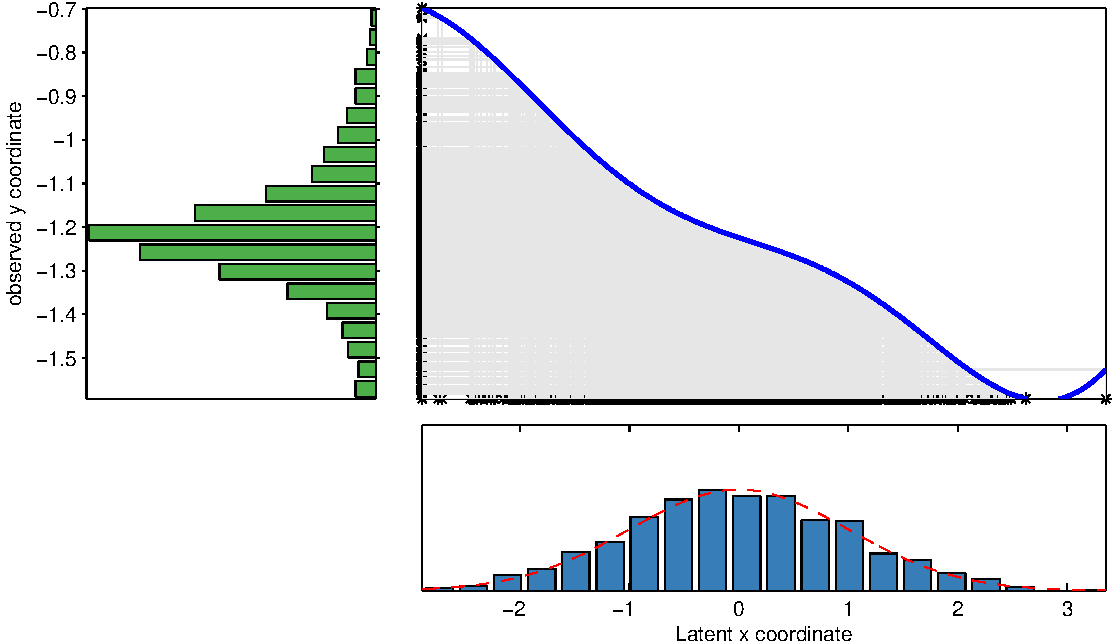
\includegraphics[width=0.8\textwidth,clip,trim=1.3cm 0.79cm 0cm 0cm]{\gplvmfiguresdir/gplvm_1d_draw_9} } &
\raisebox{3cm}{\rotatebox{90}{Warped density: $p(y)$}} \\
\qquad \qquad \qquad Latent density: $p(x)$ & 
\end{tabular}
\caption[One-dimensional Gaussian process latent variable model]{
A draw from a one-dimensional Gaussian process latent variable model. 
\emph{Bottom:} the density of a set of samples from a 1D Gaussian, specifying the distribution $p(x)$ in the latent space.
\emph{Top Right:} A function $y = f(x)$ drawn from a \gp{} prior.
Grey lines show points being mapped through $f$.
\emph{Left:} A nonparametric density $p(y)$ defined by warping the latent density through the sampled function.} 
\label{fig:oned-gplvm}
\end{figure}



\begin{figure}[t]
\centering
\begin{tabular}{ccc}
Latent space $p(\vx)$ & & Observed space $p(\vy)$ \\
\fbox{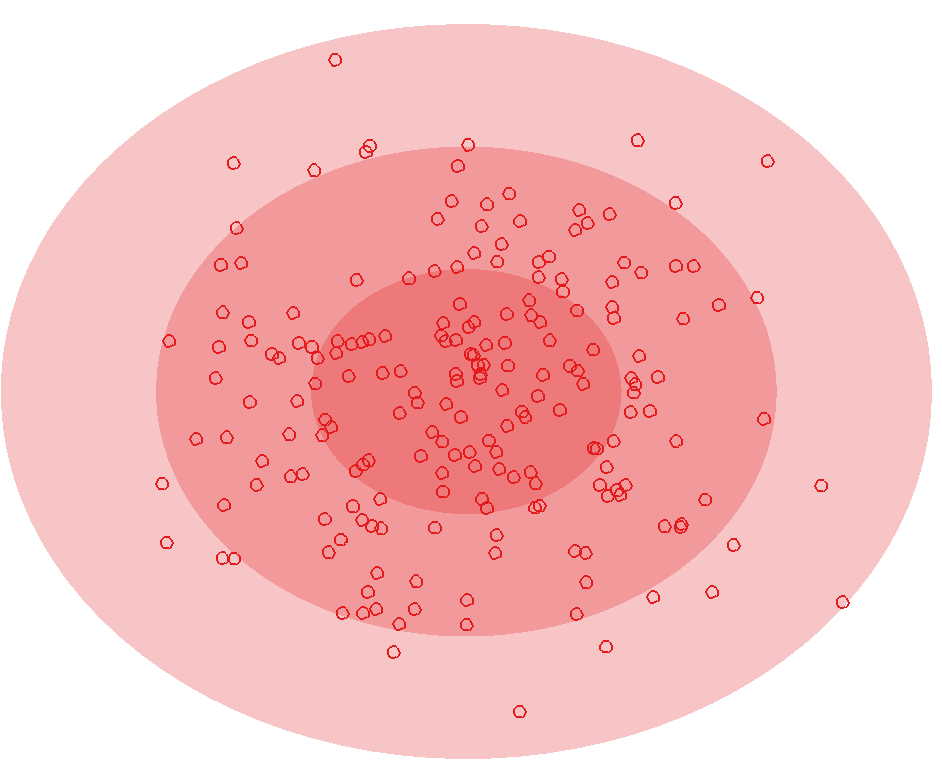
\includegraphics[height=15em,width=15em]{\gplvmfiguresdir/gplvm-latent-crop}} &
\raisebox{7em}{$\overset{ \textstyle \vf(\vx)}{ \mathlarger{\mathlarger{\mathlarger{\mathlarger{\mathlarger{ \rightarrow}}}}}}$} &
\fbox{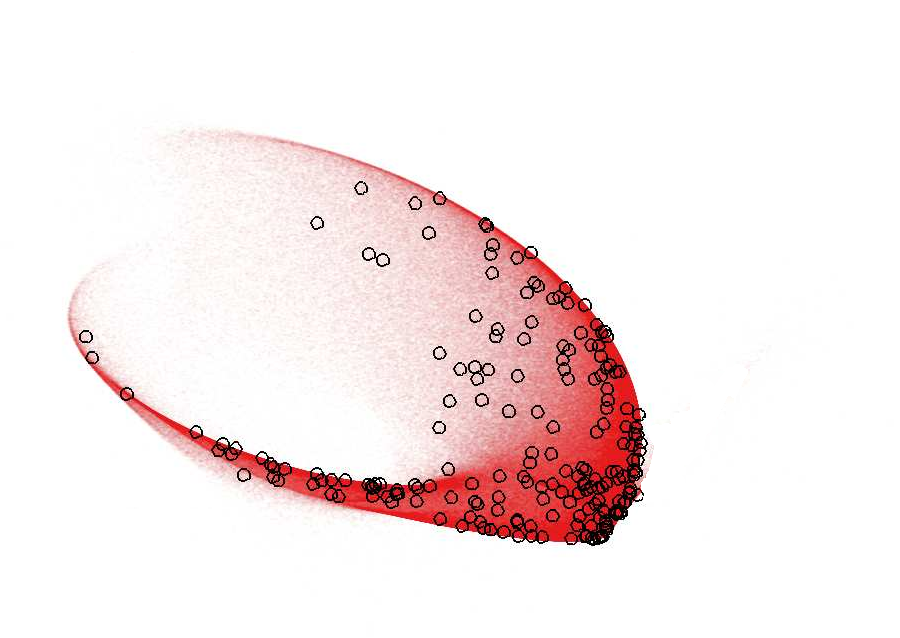
\includegraphics[height=15em,width=15em]{\gplvmfiguresdir/gplvm-draw-crop}}
\end{tabular}
\caption[Two-dimensional Gaussian process latent variable model]{A draw from a multi-dimensional Gaussian process latent variable model.
\emph{Left:} Isocontours and samples from a 2D Gaussian, specifying the distribution $p(\vx)$ in the latent space. 
\emph{Right:} Observed density $p(\vy)$ has a nonparametric shape, defined by warping the latent density through a function drawn from a \gp{} prior.}  
\label{fig:twod-gplvm}
\end{figure}



The \iwmm{} can be viewed as an extension of the Gaussian process latent variable model (\gplvm{})~\citep{lawrence2004gaussian}, a probabilistic model of nonlinear manifolds.
The \gplvm{} smoothly warps a Gaussian density into a more complicated distribution, using a draw from a \gp{}.
Usually, we think of the Gaussian density as living in a ``latent space'' having $Q$ dimensions, and the warped density living in the observed space having $D$ dimensions.

A standard definition of the \gplvm{} is as follows:
%
\begin{align}
\textnormal{latent coordinates } \vX = (\vx_1, \vx_2, \ldots, \vx_{N})\tra & \simiid \N{\vx}{0}{\vI_Q} \\
\textnormal{warping functions } \vf = (f_1, f_2, \ldots, f_D)\tra & \simiid \GPt{0}{\kSE \kernplus \kWN} \\
\textnormal{observed datapoints } \vY = (\vy_1, \vy_2, \ldots, \vy_N)\tra & = \vf(\vX)
\end{align}


%Suppose that we have a set of observations
%$\vY = (\vy_1,\ldots,\vy_N)\tra$,
%where $\vy_n \in {\mathbb R}^D$,
%and they are associated with a set of latent coordinates
%$\vX = (\vx_1,\ldots,\vx_{N})\tra$,
%where $\vx_n \in {\mathbb R}^Q$.
%The \gplvm{} assumes that observations are generated by mapping the latent coordinates through a set of smooth functions, over which Gaussian process priors are placed.
Under the \gplvm{}, the probability of observations given the latent coordinates integrating out the mapping functions, is simply a product of multivariate normals:
\begin{align}
p(\vY | \vX, \vtheta) 
& = \prod_{d=1}^D p(\vY_{:,d} | \vX, \vtheta) = \prod_{d=1}^D \N{\vY_{:,d}}{0}{\vK_\vtheta} \\ 
& = (2 \pi)^{-\frac{DN}{2}}  |\vK|^{-\frac{D}{2}} \exp \left( -\frac{1}{2} {\rm tr}( \vY\tra \vK\inv \vY) \right),
\label{eq:py_x}
\end{align}
%where $\vK$ is the $N \times N$ covariance matrix defined 
%by the kernel function $k(\vx_{n},\vx_{m})$,
where $\vtheta$ are the kernel parameters and $\vK$ is the Gram matrix $k(\vX, \vX)$.
%In this chapter, we use an \kSE + \kWN kernel.
% with an additive noise term:
%\begin{align}
%k(\vx_{n},\vx_{m}) &= \alpha \exp\left( - \frac{1}{2 \ell^2}(\vx_n - \vx_m)\tra (\vx_n - \vx_m) \right) 
%+ \delta_{nm} \beta\inv.
%\end{align}
%where $\alpha$ is 
%$\ell$ is the length scale,
%and $\beta$ is the variance of the additive noise.
%This likelihood is simply the product of $D$ independent Gaussian process likelihoods, one for each output dimension.

Typically, the \gplvm{} is used for dimensionality reduction or visualization, and the latent coordinates are set by maximizing \eqref{eq:py_x}.
In that setting, the Gaussian prior density on $\vx$ is essentially a regularizer which keeps the latent coordinates from spreading arbitrarily far apart.  
In contrast, we integrate out the latent coordinates, and the \iwmm{} places a more flexible parameterization on $p(\vx)$ than a single isotropic Gaussian.
Just as the \gplvm{} can be viewed as a manifold learning algorithm, the \iwmm{} can be viewed as learning a set of manifolds, one for each cluster.





\section{The infinite warped mixture model}
\label{sec:iwmm-definition}

\begin{figure}
\centering
\begin{tabular}{ccc}
Latent space $p(\vx)$ & & Observed space $p(\vy)$ \\
\fbox{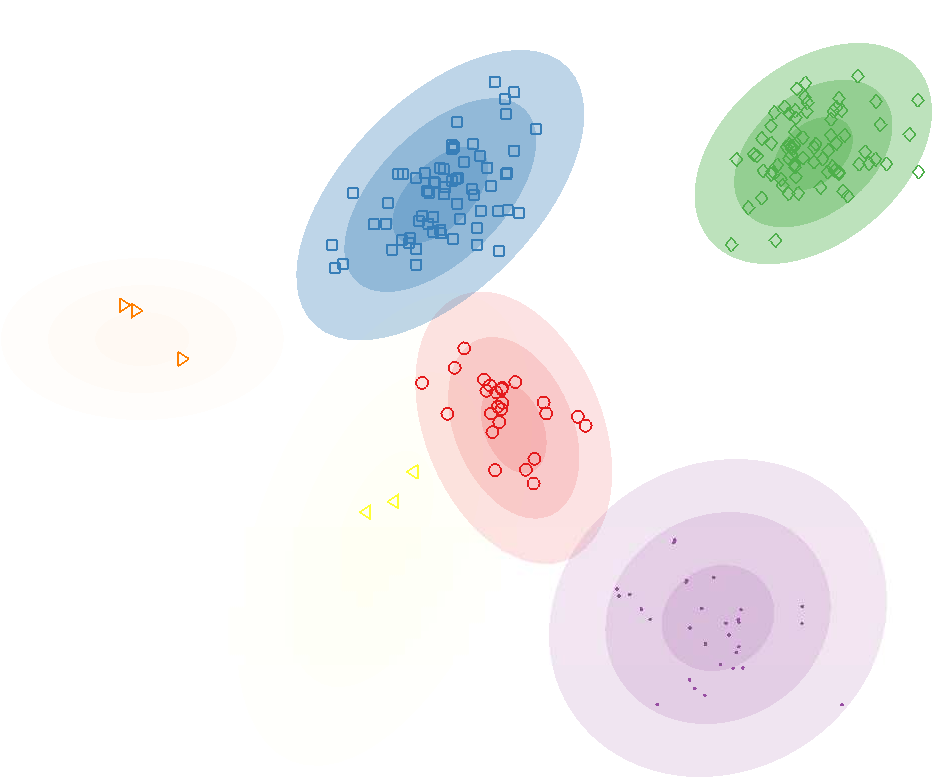
\includegraphics[trim=2em 0em 0em 0em, clip, height=15em,width=15em]{\warpedfiguresdir/iwmm_latent_N200_seed2155_darker}} &
\raisebox{7em}{$\overset{ \textstyle \vf(\vx)}{ \mathlarger{\mathlarger{\mathlarger{\mathlarger{\mathlarger{ \rightarrow}}}}}}$} &
\fbox{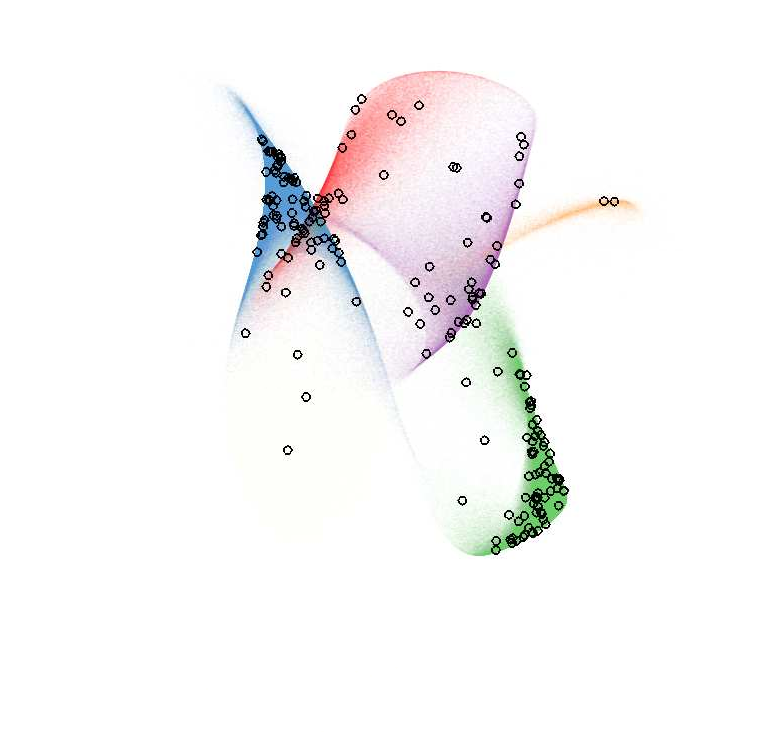
\includegraphics[trim=8em 6em 6em 2em, clip, height=15em,width=15em]{\warpedfiguresdir/iwmm_N200_seed2155_points1000000}}
\end{tabular}
\caption[A draw from the infinite warped mixture model prior]{
A sample from the \iwmm{} prior.
\emph{Left:} In the latent space, a mixture distribution is sampled from a Dirichlet process mixture of Gaussians.
\emph{Right:} The latent mixture is smoothly warped to produce a set of non-Gaussian manifolds in the observed space.}
\label{fig:generative}
\end{figure}


This section defines in detail the infinite warped mixture model (\iwmm{}).
Like the \gplvm{}, the \iwmm{} assumes a smooth nonlinear mapping from a latent density to an observed density.
The difference is that the \iwmm{} assumes that the latent density is an infinite Gaussian mixture model~(\iGMM{})~\citep{rasmussen2000infinite}:
%
\begin{align}
p(\vx ) = \sum_{c=1}^{\infty} \lambda_c \, {\cal N}(\vx|\bm{\mu}_{c},\vR_{c}\inv)
\end{align}
%
where $\lambda_{c}$, $\bm{\mu}_{c}$ and $\vR_{c}$ is the mixture weight, mean, and precision matrix of the $c^{\text{\tiny th}}$ mixture component.

The \iwmm{} can be seen as a generalization of either the \gplvm{} or the \iGMM{}.
To be precise, the \iwmm{} with a single fixed spherical Gaussian density on the latent coordinates corresponds to the \gplvm{}, while the \iwmm{} with fixed direct mapping function $f_{d}(\vx)=x_{d}$ and 
$Q=D$ corresponds to the \iGMM{}.

A flexible model of cluster shapes is required to correctly estimate the number of clusters, if those clusters do not happen to be Gaussian.
For example, a mixture of Gaussians fit to a single non-Gaussian cluster (such as one that is curved or heavy-tailed) will report that the data contains many Gaussian clusters.
% move up?





\section{Inference}
\label{sec:iwmm-inference}

As discussed in \cref{sec:useful-properties}, one of the main advantages of \gp{} priors is that, given inputs $\vX$, outputs $\vY$ and kernel parameters $\vtheta$, we can analytically integrate over functions mapping $\vX$ to $\vY$.
However, inference becomes more difficult if we introduce uncertainty about the kernel parameters, or the input locations $\vX$.
This section outlines how to infer all parameters in the \iwmm{} given only a set of observations $\vY$.
Details can be found in appendix~\ref{sec:iwmm-inference-details}.

By placing conjugate priors on the parameters of the Gaussian mixture components, we can analytically integrate out the cluster shapes, given the assignments of points to clusters.
The only remaining variables to infer are the latent points $\vX$, the cluster assignments $\vZ$, and the kernel parameters $\vtheta$.
%In particular, we'll alternate collapsed Gibbs sampling of $\vZ$ and Hamiltonian Monte Carlo sampling of $\vX$.
%
%Given $\vZ$, we can calculate the gradient of the un-normalized posterior distribution of $\vX$, integrating over warping functions.
%This gradient allows us to sample $\vX$ using Hamiltonian Monte Carlo (\HMC{}).
%
We can obtain samples from their posterior 
%$p(\vX,\vZ|\vY,\bm{\theta},\vS,\nu,\vu,r,\eta)$ 
$p(\vX,\vZ, \vtheta | \vY)$ 
by iterating two steps:
\begin{enumerate}
\item
Given the latent points $\vX$, we sample the discrete cluster memberships $\vZ$ using collapsed Gibbs sampling, integrating out the mixture parameters \eqref{eq:gibbs}.
%The conditional probability of $\vZ$ given $\vX$ is given by \eqref{eq:gibbs}.
%For each observation $n=1,\cdots,N$,
%sample the component assignment $z_{n}$ by collapsed Gibbs sampling 
\item 
Given the cluster assignments $\vZ$, we sample the continuous latent coordinates $\vX$ and kernel parameters $\vtheta$ using Hamiltonian Monte Carlo (\HMC{})~\citep[chapter 30]{mackay2003information}.
The relevant equations are given by \cref{eq:warped-hmc1,eq:warped-hmc2,eq:warped-hmc3,eq:warped-hmc4}.
\end{enumerate}

The complexity of each iteration of \HMC{} is dominated by the $\mathcal{O}(N^3)$ computation of $\vK\inv$.
This complexity could be improved by making use of an inducing-point approximation~\citep{quinonero2005unifying,snelson2006sparse}.



\subsubsection{Posterior predictive density}

One disadvantage of this model class is that its predictive density has no closed form.
To approximate the predictive density, we sample latent points from the posterior on the latent density, and map them through warpings drawn from the corresponding posterior density.
The Gaussian noise added to each observation means that each sample adds a Gaussian to the Monte Carlo estimate of the predictive density.
Details can be found in \cref{sec:iwmm-predictive-density}.
This procedure was used to generate the plots of posterior density in \cref{fig:generative,fig:warping,fig:posterior}.





\section{Related work}
\label{sec:iwmm-related-work}

The literature on manifold learning, clustering and dimensionality reduction is extensive.
This section highlights some of the most relevant related work.

\subsubsection{Extensions of the \sgplvm{}}

The \gplvm{} has been used effectively in a wide variety of applications~\citep{lawrence2004gaussian,salzmann2008local,lawrence2009non}.
The latent positions $\vX$ in the \gplvm{} are typically obtained by maximum a posteriori estimation or variational Bayesian inference~\citep{titsias2010bayesian}, placing a single fixed spherical Gaussian prior on $\vx$.

A regularized extension of the \gplvm{} which allows estimation of the dimension of the latent space was introduced by \citet{geiger2009rank}, in which the latent variables and their intrinsic dimensionality are simultaneously optimized.
The \iwmm{} can also infer the intrinsic dimensionality of nonlinear manifolds:
inferring the Gaussian covariance for each latent cluster allows the variance of irrelevant dimensions to become small.
The marginal likelihood of the latent Gaussian mixture will favor using as few dimensions as possible to describe each cluster.
In fact, because each latent cluster has a different set of parameters, each cluster can have a different effective dimension.
This allows the \iwmm{} to model manifolds of differing dimension in the observed space, as demonstrated in \cref{fig:warping}(b).

\citet{nickisch2010gaussian} considered several modifications of the \gplvm{} which model the latent density using a mixture of Gaussians centered around the latent points.
They approximated the observed density $p(\vY)$ by another mixture of Gaussians, obtained by moment-matching the latent Gaussians after they had been warped into the observed space.
Training was done by maximizing a leave-some-out predictive density.
This method had poor predictive performance compared to simple baselines, and was not have a generative clustering model.
%spherical Gaussian at each latent datapoint, and approximated the implied density in the observed space with another set of Gaussians, one for each datapoint.
%This model enjoys some of the flexibility of the \iwmm{}, but 


\subsubsection{Related linear models}
The \iwmm{} can also be viewed as a generalization of the mixture of probabilistic principle component analyzers~\citep{tipping1999mixtures}, or the mixture of factor analyzers~\citep{ghahramani2000variational}, where the linear mapping of the mixtures is generalized to a nonlinear mapping by Gaussian processes, and the number of components is infinite.


\subsubsection{Non-probabilistic methods}
There exist non-probabilistic clustering methods which can find clusters with complex shapes, such as spectral clustering~\citep{ng2002spectral} and nonlinear manifold clustering~\citep{cao2006nonlinear,elhamifar2011sparse}.
Spectral clustering finds clusters by first forming a similarity graph, then finding a low-dimensional latent representation using the graph, and finally, clustering the latent coordinates via k-means.
The performance of spectral clustering depends on parameters which are usually set manually, such as the number of clusters, the number of neighbors, and the variance parameter used for constructing the similarity graph.
The \iwmm{} infers such parameters automatically, and has no need to construct a similarity graph.
%The \iwmm{} can be viewed as a probabilistic generative model for spectral clustering, where the both methods find clusters in a nonlinearly mapped low-dimensional space.  

The kernel Gaussian mixture model~\citep{wang2003kernel} can also find non-Gaussian shaped clusters.
This model estimates a \GMM{} in the implicit infinite-dimensional feature space defined by the kernel mapping of the observed space.
%However, the kernel \GMM{} uses a fixed nonlinear mapping function, with no likelihood term that encourages the latent points to be well-modeled by a \GMM{}.
However, the kernel parameters must be set by cross-validation.
%and the data points mapped by a fixed function are not guaranteed 
%to be distributed according to a GMM.
In contrast, the \iwmm{} infers the mapping function such that the latent coordinates will be well-modeled by a mixture of Gaussians.

%The infinite mixtures of Gaussian process experts~\citep{rasmussen2002infinite}
%uses Dirichlet process and Gaussian process priors for regression problems.
%The mixture of ppca
%ppca \citep{tipping1999probabilistic}
%mixture of ppca \citep{tipping1999mixtures}
%one Gaussian process function

\subsubsection{Nonparametric cluster shapes}

To the best of our knowledge, the only other Bayesian clustering method with nonparametric cluster shapes is that of \citet{rodriguez2012univariate}, who for one-dimensional data introduce a nonparametric model of \emph{unimodal} clusters, where each cluster's density function strictly decreases away from its mode.


\subsubsection{Deep Gaussian processes}

An elegant way to construct a \gplvm{} with a more structured latent density $p(\vx)$ is to use another \gplvm{} to model the latent coordinates $\vX$.
This latent \gplvm{} can have another \gplvm{} modeling its latent space, etc.
This is exactly the model class considered by \citet{damianou2012deep}, who also test to what extent each layer's latent representation implicitly forms clusters.
They found that when modeling \MNIST{} hand-written digits, nearest-neighbour classification performed best in the 4th layer of a 5-layer deep nested \gplvm{}, suggesting that the latent density might have  been implicitly forming clusters at that level.


\section{Experimental results}
\label{sec:iwmm-experiments}

\subsection{Synthetic datasets}
Figure~\ref{fig:warping} demonstrates the proposed model on four synthetic datasets.
%The top row of Figure~\ref{fig:warping} shows the two-dimensional observed data points (unlabeled) and the non-Gaussian clusters inferred by the \iwmm{}.
% The bottom row shows the latent coordinates and Gaussian components in the latent space inferred by the \iwmm{}.
% Each plot shows a single sample from the Markov chain.
%
\def\inclatentpic#1{\fbox{\includegraphics[width=0.22\columnwidth, height=0.2\columnwidth]{\warpedfiguresdir/#1}}}
\begin{figure}[t]
\centering
{\tabcolsep=0.3em
\begin{tabular}{cccc}
\multicolumn{4}{c}{Observed space} \\
\inclatentpic{spiral2_x3_observed_coordinates_epoch5000} &
\inclatentpic{halfcircles_N100K3_x3_observed_coordinates_epoch5000} &
\inclatentpic{circles_N50K2_x3_observed_coordinates_epoch5000} &
\inclatentpic{pinwheel_N50K5_x3_observed_coordinates_epoch5000} \\
$\uparrow$ & $\uparrow$ & $\uparrow$ & $\uparrow$ \\ 
\inclatentpic{spiral2_x_latent_coordinates_epoch5000} &
\inclatentpic{halfcircles_N100K3_x_latent_coordinates_epoch5000} &
\inclatentpic{circles_N50K2_x_latent_coordinates_epoch5000} &
\inclatentpic{pinwheel_N50K5_x_latent_coordinates_epoch5000} \\
\multicolumn{4}{c}{Latent space} \\
(a) 2-curve & (b) 3-semi & (c) 2-circle & (d) Pinwheel \\
\end{tabular}}
\caption[Recovering clusters on synthetic data]{
\emph{Top row:} The observed unlabeled data points (black), and the cluster densities inferred by the \iwmm{} (colors).
\emph{Bottom row:} Latent coordinates and Gaussian components from a single sample from the posterior.
Each point in the latent space corresponds to a point in the observed space.}
\label{fig:warping}
\end{figure}
%
None of these four datasets can be appropriately clustered by Gaussian mixture models (\GMM{}).
For example, consider the 2-curve data shown in \Cref{fig:warping}(a), where 100 data points lie in each of two curved lines in a two-dimensional observed space.
%as shown at the top row of .
A \GMM{} with two components cannot separate the two curved lines, while a \GMM{} with many components could separate the two lines only by breaking each line into many clusters. 
In contrast, the \iwmm{} represents the two non-Gaussian clusters in the observed space by two Gaussian-shaped clusters in the latent space.
\Cref{fig:warping}(b) shows a simple extension to three non-linearly-seperable clusters.
%The \iwmm{} separated the two curved lines by nonlinearly warping two Gaussians from the latent space to the observed space.

\Cref{fig:warping}(c) shows an interesting manifold learning challenge: a dataset consisting of two concentric circles.
The outer circle is modeled in the latent space by a Gaussian with one effective degree of freedom.
This linear topology is fit to the outer circle in the observed space by bending the two ends until they cross over.
In contrast, the sampler fails to discover the 1D topology of the inner circle, modeling it with a 2D manifold instead.
This example demonstrates that each cluster in the \iwmm{} manifold can have a different effective dimension.

\Cref{fig:warping}(d) shows a five-armed variant of the pinwheel dataset of \citet{adams2009archipelago}, generated by warping a mixture of Gaussians into a spiral.
This generative process closely matches the assumptions of the \iwmm{}.
Unsurprisingly, the \iwmm{} is able to recover an anologous latent structure, and its predictive density follows the observed data manifolds.





\subsection{Clustering face images}

We also examined our model's ability to model images without pre-processing.
We constructed a dataset consisting of 50 greyscale 32x32 pixel images of two individuals from the \UMIST{} faces dataset~\citep{umistfaces}.
Both series of images show a person turning his head to the right to varying degrees.

\begin{figure}[h!]
\centering
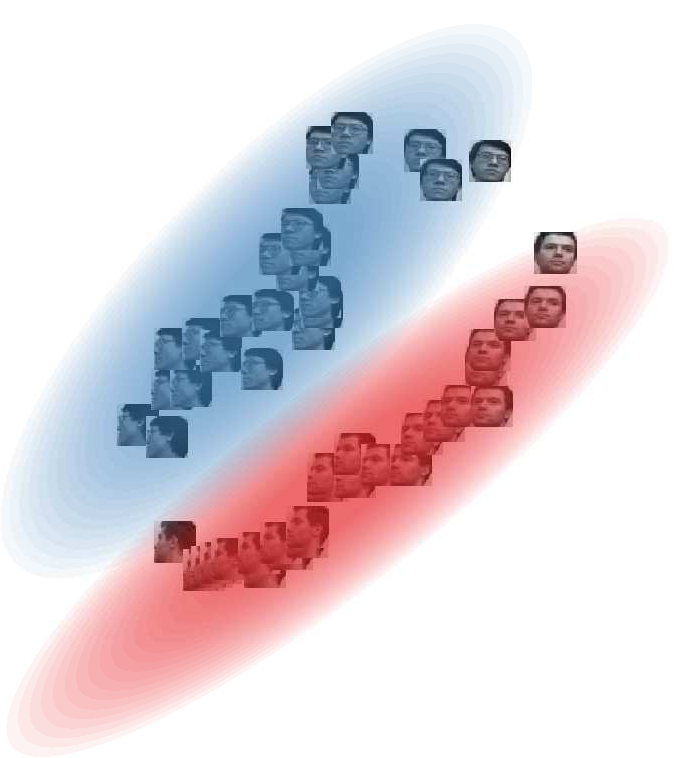
\includegraphics[width=0.5\columnwidth]{\warpedfiguresdir/faces2}
\caption[Latent clusters of face images]{A sample from the 2-dimensional latent space when modeling a series of 32x32 face images.
Images are rendered at their latent 2D coordinates.
Our model correctly discovers that the data consists of two separate manifolds, both approximately one-dimensional, which both share the same head-turning structure.}
\label{fig:faces}
\end{figure}

\Cref{fig:faces} shows a sample from the posterior over latent coordinates as well as the density model, with each image rendered at its location in the latent space.
The model has recovered three relevant, interpretable features of the dataset:
First, that there are two distinct faces.
Second, that each set of images lies approximately along a smooth one-dimensional manifold.
Third, that the two manifolds share roughly the same structure: the front-facing images of both individuals lie close to one another, as do the side-facing images.






\subsection{Density estimation}

\begin{figure}[ht!]
\centering
\begin{tabular}{cc}
(a) \iwmm{} & (b) \gplvm{} \\
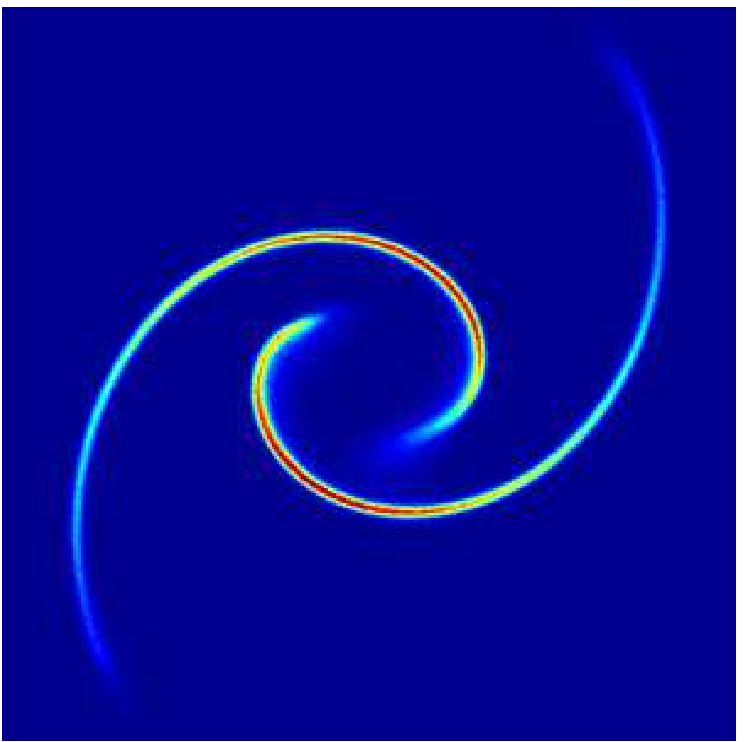
\includegraphics[width=0.4\columnwidth]{\warpedfiguresdir/result_spiral2_ydistribution} &
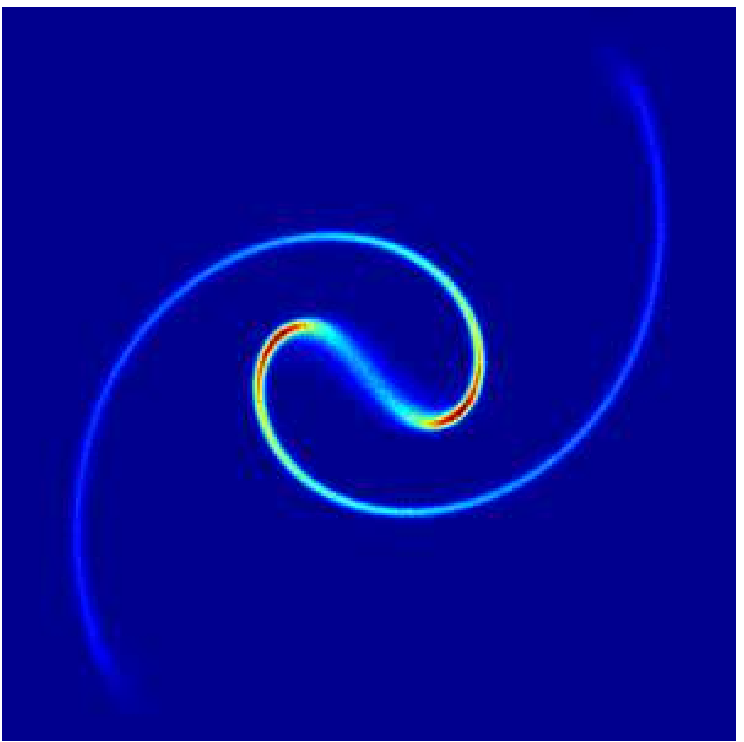
\includegraphics[width=0.4\columnwidth]{\warpedfiguresdir/result_spiral2all_gplvm_ydistribution}
\end{tabular}
\caption[Comparing density estimates of between the \sgplvm{} and the \siwmm{}]{
\emph{Left:} Posterior density inferred by the \iwmm{} in the observed space, on the 2-curve data.
\emph{Right:} Posterior density inferred by the \iwmm{} with one component, a model equivalent to a fully-Bayesian \gplvm{}.}
\label{fig:posterior}
\end{figure}

\Cref{fig:posterior}(a) shows the posterior density in the observed space inferred by the \iwmm{} on the 2-curve data, computed using 1000 samples from the Markov chain.
The two separate manifolds of high density implied by the two curved lines was recovered by the \iwmm{}.  
Note also that the density along the manifold varies along with the density of data, shown in \cref{fig:warping}(a).  
%The warped densities output by our model are actually a richer representation than simply a set of manifolds, since they also define a density at each point in the observed space.
%The density computed using multiple samples from MCMC is clearer than the density computed from a single sample shown at the bottom of Figure~\ref{fig:warping} (a).

This result can be compared to a special case of our model with only a single Gaussian in the latent space, equivalnt to a fully-Bayesian \gplvm{}.
\Cref{fig:posterior}(b) shows that the single-cluster variant of the \iwmm{} posterior is forced to place significant density connecting the two clusters, since it has to reproduce the observed density manifold by warping a single Gaussian.




\def\incwarpmixpic#1{\fbox{\includegraphics[width=0.22\columnwidth, height=0.2\columnwidth]{\warpedfiguresdir/#1}}}
\begin{figure}
\centering
{\tabcolsep=0.3em
\begin{tabular}{cccc}
\incwarpmixpic{spiral2all_o_latent_coordinates_epoch1}&
\incwarpmixpic{spiral2all_o_latent_coordinates_epoch500} & 
\incwarpmixpic{spiral2all_o_latent_coordinates_epoch1800}&
\incwarpmixpic{spiral2all_o_latent_coordinates_epoch3000}\\
(a) Initialization & (b) Iteration 500 & (c) Iteration 1800 & (d) Iteration 3000 \\
\end{tabular}}
\caption[A visualization of a sampler for the \siwmm{}]{The inferred infinite GMMs over iterations in the two-dimensional latent space with the \siwmm{} using the 2-curve data. Labels indicate the number of iterations of the sampler, and the color of each point represents its ordering in the observed coordinates.}
\label{fig:infer}
\end{figure}



\subsection{Mixing}

An interesting side-effect of learning the number of latent clusters is that this added flexibility can help the sampler escape local minima.
\Cref{fig:infer} shows the samples of the latent coordinates and clusters of the \iwmm{} over a single Markov chain modeling the 2-curve data.
\Cref{fig:infer}(a) shows the latent coordinates initialized at the observed coordinates, starting with one latent component.
After 500 iterations, each curved line was modeled by two components.
After 1800 iterations, the left curved line was modeled by a single component.
After 3000 iterations, the right curved line was also modeled by a single component, and the dataset was appropriately clustered.
This configuration was relatively stable, and a similar state was found at the 5000th iteration.
%In this way, the \iwmm{} can find latent coordinates
%by flexibly changing the number of components.


\subsection{Visualization}
Next, we briefly investigate the potential of the \iwmm{} for low-dimensional visualization of data.
%
\def\incdensitypic#1{\fbox{\includegraphics[width=0.3\columnwidth, height=0.3\columnwidth]{\warpedfiguresdir/#1}}}
\begin{figure}[ht!]
\centering
{\tabcolsep=0.3em
\begin{tabular}{cc}
\incdensitypic{spiral2all_o_latent_coordinates} &
\incdensitypic{spiral2all_wm2_o_latent_coordinates} \\
%\incdensitypic{spiral2_gplvm2_o_latent_coordinates} &
%\incdensitypic{spiral2_fixedgaussgplvm_o_latent_coordinates}\\
(a) \iwmm{} & (b) \iwmm{} ($C=1$) %& (c) \gplvm{} & (d) \vbgplvm{}
\end{tabular}}
\caption[Comparison of latent coordinate estimates]{Latent coordinates of the 2-curve data, estimated by two different methods.
% by (a) \iwmm{}, (b) \iwmm{} ($C=1$), (c) \gplvm{}, and (d) Bayesian \gplvm{}.
}
\label{fig:latent}
\end{figure}
%
\Cref{fig:latent}(a) shows the latent coordinates obtained by averaging over 1000 samples from the posterior of the \iwmm{}.
Because rotating the latent coordinates does not change their probability, simple averaging may not be an adequate way to summarize the posterior.
However, we show this result in order to show the characteristics of latent coordinates obtained by the \iwmm{}.
The estimated latent coordinates are clearly separated, and they form two straight lines.
This result is an example of the \iwmm{} recovering the original topology of the data before it was warped.

For comparison, \Cref{fig:latent}(b) shows the latent coordinates estimated by the \iwmm{} when forced to use a single cluster (again, equivalent to a fully-Bayesian \gplvm{}).
In this case, the latent coordinates lie in two sections of a single straight line.
%\Cref{fig:latent}(c) shows the result of standard \MAP{} estimation in the \gplvm{}, and \cref{fig:latent}(d) shows the result of variational Bayesian inference of \citet{titsias2010bayesian}.
%These methods did not unfold the two curved lines, since the effective dimension of their latent representation is fixed beforehand.
%because in these models, no force to favor forming a low-dimensional manifold.
%In contrast, the \iwmm{} effectively formed a low-dimensional representation in the latent space. 

Regardless of the dimension of the latent space, the \iwmm{} will tend to model each cluster with as low-dimensional a Gaussian as possible, 
%This is because, if the data in a cluster can be made to lie in a low-dimensional plane, 
since a narrowly-shaped Gaussian will assign the latent coordinates much higher likelihood than a spherical Gaussian.

\subsection{Clustering performance}
We more formally evaluated the density estimation and clustering performance of the proposed model using four real datasets: iris, glass, wine and vowel, obtained from \LIBSVM{} multi-class datasets~\citep{chang2011libsvm}, in addition to the four synthetic datasets shown above: 2-curve, 3-semi, 2-circle and pinwheel~\citep{adams2009archipelago}.
The statistics of these datasets are summarized in \Cref{tab:statistics}.
%
\begin{table}[ht!]
\centering
\caption[Datasets used for evaluation of the \siwmm{}]
{Statistics of the datasets used for evaluation.}
\label{tab:statistics}
\begin{tabular}{rrrrrrrrr}
\hline
 & 2-curve & 3-semi & 2-circle & pinwheel & iris & glass  & wine  & vowel  \\
\hline
samples: $N$ & 100 & 300 & 100 & 250 & 150 & 214 & 178 & 528 \\
dimension: $D$ & 2 & 2 & 2 & 2 & 4 & 9 & 13 & 10 \\
num. clusters: $C$ & 2 & 3 & 2 & 5 & 3 & 7 & 3 & 11 \\
\hline
\end{tabular}
\end{table}
%
In each experiment, we show the results of ten-fold cross-validation.
Results in bold are not significantly different from the best performing method in each column according to a paired t-test.
%In each experiment, 10\% of the data was used for testing.
%
%
%We used two evaluation measurements: test point likelihood and Rand index
%for evaluating in terms of density estimation performance
%and clustering performance, respectively.
% the Gaussian-Wishart prior is quite different in these cases, placing more mass on higher-dimensional manifolds when the dimension of the latent space is high.  Placing a hyper-prior allowing the concentration parameter $\eta$ to vary may shrink these differences.

\begin{table}[ht!]
\centering
\caption[Clustering performance comparison]
{Average Rand index for evaluating clustering performance.}
\label{tab:rand}
\begin{tabular}{lrrrrrrrr}
\hline
 & 2-curve & 3-semi & 2-circle & Pinwheel & Iris  & Glass  & Wine  & Vowel  \\
\hline
iGMM & $0.52$ & $0.79$ & $0.83$ & $0.81$ & $0.78$ & $0.60$ & $0.72$ & $\mathbf{0.76}$ \\
iWMM(Q=2) & $\mathbf{0.86}$ & $\mathbf{0.99}$ & $\mathbf{0.89}$ & $\mathbf{0.94}$ & $\mathbf{0.81}$ & $\mathbf{0.65}$ & $0.65$ & $0.50$ \\
iWMM(Q=D) & $\mathbf{0.86}$ & $\mathbf{0.99}$ & $\mathbf{0.89}$ & $\mathbf{0.94}$ & $0.77$ & $0.62$ & $\mathbf{0.77}$ & $\mathbf{0.76}$ \\
\hline
\end{tabular}
\end{table}
%
\Cref{tab:rand} compares the clustering performance of the \iwmm{} with the \iGMM{}, quantified by the Rand index~\citep{rand1971objective}, which measures the correspondence between inferred clusters and true clusters.
Since the manifold on which the observed data lies can be at most $D$-dimensional, we set the latent dimension $Q$ equal to the observed dimension $D$ in \iwmm{}s.
We also included the $Q = 2$ case in an attempt to characterize how much modeling power is lost by forcing the latent representation to be visualizable. 

%The \iGMM{} is another probabilistic generative model commonly used for clustering, which can be seen as a special case of the \iwmm{} in which the Gaussian clusters are not warped.  
These experiments were designed to measure the extent to which nonparametric cluster shapes helped to estimate meaningful clusters.
To eliminate any differences due to different inference procedures, we used identical code for the \iGMM{} and \iwmm{}, the only difference being that the warping function was set to the identity $\vx = \vy$.
%When the latent dimensionality was set to two ($Q=2$), clustering performance was degraded.% did not work well
%because information was lost by reducing the dimensionality.
Both variants of the \iwmm{} usually outperformed the \iGMM{} on this measure.


\subsection{Density estimation}

Next, we compared the \iwmm{} in terms of predictive density against kernel density estimation (\KDE{}) and the (\iGMM{}).
For \KDE{}, the kernel width was estimated by maximizing the leave-one-out density.

Although all these methods are consistent density estimators, we expect the \iwmm{} to have an advantage for finite datasets, since its density contours can follow the data density.
%With WM and \iwmm{}, we set the dimensionality of the latent space
%at that of the observed space $Q=D$ or $Q=2$.
%We include the $Q=2$ case in order to attempt to quantify the 
%The proposed models achieved higher test log likelihoods than the KDE, MPW
%
\Cref{tab:likelihood} lists average test log likelihoods.
%
\begin{table}[ht!]
\centering
\caption[Predictive likelihood comparison]
{Average test log-likelihoods for evaluating density estimation performance.}
\label{tab:likelihood}
\begin{tabular}{lrrrrrrrr}
\hline
& 2-curve & 3-semi & 2-circle & Pinwheel & Iris  & Glass  & Wine  & Vowel  \\
\hline 
KDE & $-2.47$ & $-0.38$ & $-1.92$ & $-1.47$ & $\mathbf{-1.87}$ & $1.26$ & $-2.73$ & $\mathbf{6.06}$ \\
iGMM & $-3.28$ & $-2.26$ & $-2.21$ & $-2.12$ & $-1.91$ & $3.00$ & $\mathbf{-1.87}$ & $-0.67$ \\
\iwmm{}(Q=2) & $\mathbf{-0.90}$ & $\mathbf{-0.18}$ & $\mathbf{-1.02}$ & $\mathbf{-0.79}$ & $\mathbf{-1.88}$ & $\mathbf{5.76}$ & $\mathbf{-1.96}$ & $\mathbf{5.91}$ \\
\iwmm{}(Q=D) & $\mathbf{-0.90}$ & $\mathbf{-0.18}$ & $\mathbf{-1.02}$ & $\mathbf{-0.79}$ & $\mathbf{-1.71}$ & $\mathbf{5.70}$ & $-3.14$ & $-0.35$ \\
\hline
\end{tabular}
\end{table}


The \iwmm{} usually achieved higher test likelihoods than the \KDE{} and the \iGMM{}.
%The \iwmm{} achieved better performance than WM for each latent dimensionality,
%except on the wine dataset.
% This result indicates that it is important to assume an infinite mixture model in the latent space for density estimation.%, and that even a fully Bayesian version of the \gplvm{} is not necessarily a good density model.
%
The sometimes large differences between performance in the $D = 2$ case and the $D = Q$ case may be attributed to the fact that when the latent dimension is high, it requires many samples from the latent distribution to produce an accurate estimate of the posterior density at the test locations.
This difficulty in inference might be solved by using a warping with back-constraints~\citep{Lawrence06localdistance}, that would allow a more direct evaluation of the density at a given point in the observed space.




\subsubsection{Source code}
Code to reproduce all the above figures and experiments is available at \\\url{github.com/duvenaud/warped-mixtures}.


\section{Conclusions}

This chapter introduced a simple generative model of non-Gaussian density manifolds which can infer nonlinearly separable clusters, low-dimensional representations of varying dimension per cluster, and density estimates which smoothly follow the contours of each cluster.
We then introduced a sampler for this model which integrates out both the cluster parameters and the warping function exactly.
%We further demonstrated that allowing non-parametric cluster shapes improves clustering performance over the Dirichlet process Mixture of Gaussians.

%Relatively flexible nonparametric clustering models already exist
Non-probabilistic methods such as spectral clustering can also produce nonparametric cluster shapes, but usually lack principled methods for setting kernel parameters, the number of clusters, and the implicit dimension of the learned manifolds, other than by cross-validation.
This chapter shows that using a fully generative model allows most model choices to be determined automatically.

Many methods have been proposed which can perform some combination of clustering, manifold learning, density estimation and visualization.
We demonstrated that a simple but flexible probabilistic generative model can perform well at all these tasks.

%Since the proposed model is generative, it can also be extended to handle missing data, integrate with other probabilistic models, and use other families of distributions for the latent components.


\section{Future work}

%One design decision which may be worth revisiting is the use the same warping for all mixture components.  It would be simple, and typically faster, to use a separate set of GPs to model the warping of each latent cluster.  

\subsubsection{More sophisticated latent density models}
The Dirichlet process mixture of Gaussians in the latent space of our model could easily be replaced by a more sophisticated density model, such as a hierarchical Dirichlet process~\citep{teh2006hierarchical}, or a Dirichlet diffusion tree~\citep{neal2003density}.
Another straightforward extension of our model would be making inference more scalable by using sparse Gaussian processes~\citep{quinonero2005unifying,snelson2006sparse} or more advanced Hamiltonian Monte Carlo methods~\citep{zhang2011quasi}.


\subsubsection{A finite cluster count model}
\citet{miller2013inconsistent} note that the Dirichlet process assumes infinitely many clusters, and that estimates of the number of clusters in a dataset based on Bayesian inference are inconsistent under this model.
They propose a consistent alternative which also allows efficient Gibbs sampling, called the mixture of finite mixtures.
Replacing the Dirichlet process with a mixture of finite mixtures would improve the conistency properties of the \iwmm{} in most applications.


%As mentioned above, another natural alternative would be to use nested \gplvm{} density models, recovering a deep \gp{} latent variable model.
%An interesting open question is whether 
%TODO: talk about deep GPs


\subsubsection{Semi-supervised learning}

An interesting but more complex extension of the \iwmm{} would be a semi-supervised version of the model.
The \iwmm{} could allow label propagation along regions of high density in the latent space, even if the individual points in those regions are stretched far apart along low-dimensional manifolds in the observed space.
Another natural extension would be to allow a separate warping for each cluster, producing a mixture of warped Gaussians, rather than a warped mixture of Gaussians.% which would also improve inference speed.




\subsubsection{Learning the topology of data manifolds}

Some datasets naturally live on manifolds which are not simply connected.
For example, motion capture data or video of a person walking in a circle naturally lives on a torus, with one coordinate specifying the phase of the person's step, and another specifying how far around the circle they've walked.

%What if we were to use the structured kernels of \cref{ch:kernels,ch:grammar} to specify the prior on warpings?
As shown in \cref{sec:topological-manifolds}, using structured kernels to specify the warping of a latent space gives rise to interesting topologies on the observed density manifold.
If a suitable method for computing the marginal likelihood of a \gplvm{} is available, an automatic search similar to that described in \cref{ch:grammar} would be possible, automatically finding the topology of the data manifold.


% Todo:  Cite paper from Jeff's talk that suggests using DP mixtures to estimate the number of clusters.


%This model is 

%Table \ref{tab:count} shows the inferred number of components
%by the iGMM and \iwmm{}.
%With the synthetic data sets, 
%the number of components inferred by the \iwmm{} was 
%
%\begin{table*}[t!]
%\centering
%\caption{Average inferred number of components.}
%\label{tab:count}
%\begin{tabular}{lrrrrrrrr}
%\hline
% & 2-curve & 3-semi & 2-circle & Pinwheel & Iris  & Glass  & Wine  & Vowel  \\
%\hline
%iGMM & 2.7 & 4.5 & 3.8 & 4.2 & 2.0 & 2.3 & 2.7 & 5.0 \\ 
%iWMM($Q=2$) & 2.2 & 3.0 & 3.2 & 4.6 & 2.6 & 3.7 & 3.1 & 2.8 \\
%iWMM($Q=D$) & 2.2 & 3.0 & 3.2 & 4.6 & 2.0 & 2.8 & 5.9 & 5.1 \\ 
%\hline
%true & 2 & 3 & 2 & 5 & 3 & 7 & 3 & 11 \\
%\hline
%\end{tabular}
%\end{table*}
%


%In contrast to the many somewhat ad-hoc clustering, manifold learning, density estimation, and visualization methods introduced recently, we show that a simple generative model can perform well at all of these tasks.

%We introduced a nonparametric Bayesian clustering method capable of inferring nonlinearly separable clusters.
%In the experiments, we demonstrated that our model is effective for density estimation, and performs much better than infinite Gaussian mixture models at discovering meaningful clusters.


%\subsection*{Acknowledgements}
%The authors would like to thank Dominique Perrault-Joncas, Carl Edward Rasmussen, and Ryan Prescott Adams for helpful discussions.
%\pagebreak

%\section{Open Questions}

%\subsubsection{How can we extend this model to handle heavy-tailed clusters?}


\outbpdocument{
\bibliographystyle{plainnat}
\bibliography{references.bib}
}


